% !TEX program = xelatex
\documentclass[12pt]{article}

\usepackage[letterpaper,margin=1in]{geometry}
\usepackage{iftex}
\ifPDFTeX
  \usepackage[T1]{fontenc}
  \usepackage{newtxtext}
  \newcommand{\headingfont}{\normalfont}
\else
  \usepackage[no-math]{fontspec}
  \setmainfont{Times New Roman}
  \IfFontExistsTF{Microsoft YaHei}{
    \setsansfont{Microsoft YaHei}
  }{
    \IfFontExistsTF{Heiti SC}{
      \setsansfont{Heiti SC}
    }{
      \setsansfont{Arial}
    }
  }
  \IfFontExistsTF{Courier New}{
    \setmonofont{Courier New}[Scale=MatchLowercase]
  }{
    \setmonofont{Menlo}[Scale=MatchLowercase]
  }
  \newcommand{\headingfont}{\sffamily}
\fi
\usepackage{amsmath}
\usepackage{newtxmath}
\usepackage{booktabs}
\usepackage{array}
\usepackage{caption}
\usepackage{enumitem}
\usepackage{graphicx}
\usepackage{placeins}
\usepackage{setspace}
\usepackage{titlesec}
\usepackage[hidelinks]{hyperref}

\setlength{\parindent}{0pt}
\setlength{\parskip}{7pt}
\setstretch{1.08}
\raggedbottom
\renewcommand{\arraystretch}{1.15}
\setlength{\tabcolsep}{5pt}
\renewcommand{\thefigure}{S\arabic{figure}}
\renewcommand{\thetable}{S\arabic{table}}
\renewcommand{\tablename}{Table}
\renewcommand{\figurename}{Figure}
\newcolumntype{L}[1]{>{\raggedright\arraybackslash}p{#1}}

\captionsetup[table]{
  font=normalsize,
  labelfont=normalfont,
  labelsep=period,
  justification=raggedright,
  singlelinecheck=false,
  skip=4pt
}
\captionsetup[figure]{
  font=normalsize,
  labelfont=normalfont,
  labelsep=period,
  justification=raggedright,
  singlelinecheck=false,
  skip=6pt
}

\titleformat{\section}
  {\headingfont\Large\bfseries}
  {\thesection.}
  {0.35em}
  {}
\titleformat{\subsection}
  {\headingfont\large\bfseries}
  {\thesubsection}
  {0.45em}
  {}
\titlespacing*{\section}{0pt}{18pt}{12pt}
\titlespacing*{\subsection}{0pt}{14pt}{7pt}

\begin{document}

\thispagestyle{plain}
\vspace*{0pt}

{\headingfont\Large Supplementary Information for\par}

\vspace{0.55in}

{\headingfont\Large PepALD: Macrocyclic Peptide Generation via\\ AutoRegressive Latent Diffusion\par}

\vspace{0.35in}

First Author\textsuperscript{1,*}, Second Author\textsuperscript{2} and Third Author\textsuperscript{2,*}

\vspace{0.20in}

\textsuperscript{1}Department, Institution, City, Post Code, Country\\
\textsuperscript{2}Department, Institution, City, Post Code, Country

\textsuperscript{*}To whom correspondence should be addressed.

\vspace{0.35in}

This file contains the following information:

\begin{enumerate}[label=\arabic*., leftmargin=1.0in, labelsep=0.25in, itemsep=1pt, topsep=6pt]
\item Implementation, data processing, and vocabulary.
\item Model training and generation settings.
\item Reference-model and property-scoring protocols.
\item Docking protocol.
\item Target-specific WP-DPO implementation settings.
\item R-group-aware ring-bond predictor details.
\item Robust reward normalization.
\item Generation-quality metrics.
\item Preference-pair construction for WP-DPO.
\item Hybrid-decoder fusion-weight sweep.
\item Permeability-training trajectory.
\end{enumerate}

\clearpage

\section{Implementation, data processing, and vocabulary}
\label{supsec:implementation_data}

All PepALD experiments used the same processed HELM representation, monomer library, and Uni-Mol embedding files.
The ChEMBL32 pretraining corpus was extracted from the \texttt{HELM} column of the ChEMBL32 biotherapeutics table by retaining non-empty HELM strings.
The CycPeptMPDB corpus was normalized by mapping all peptide polymer identifiers to \texttt{PEPTIDE1}, followed by duplicate removal.
For the permeability-enriched prior, the merged prior table was ranked by the random-forest permeability predictor and the top 1,000 entries were used for an additional cyclic-only fine-tuning stage.
The resulting data and vocabulary sizes are summarized in Table~\ref{tab:sup_data_vocab}.

\begin{table}[htbp]
\centering
\small
\caption{Processed data sources and vocabulary used in PepALD.}
\label{tab:sup_data_vocab}
\begin{tabular}{L{0.29\textwidth}L{0.62\textwidth}}
\toprule
Item & Implementation details \\
\midrule
ChEMBL32 pretraining corpus & \path{data/processed/helm_sequences_chembl32.txt}; 20,783 non-empty HELM sequences extracted from the ChEMBL32 \texttt{HELM} column. \\
CycPeptMPDB cyclic corpus & \path{data/processed/helm_sequences_cycpeptmpdb.txt}; 7,348 unique HELM sequences after peptide-polymer identifier normalization to \texttt{PEPTIDE1} and duplicate removal. \\
Permeability-prior corpus & \path{data/processed/prior_data_sorted_1000.csv}; top 1,000 entries selected by predicted permeability from the merged prior table. \\
Monomer library & \path{data/processed/monomer_library.csv}; 3,104 peptide monomer entries with curated CXSMILES and R-group availability. The CSV has 3,105 lines including the header. \\
HELM vocabulary & \path{data/processed/helm_vocab.json}; 3,105 tokens in total, consisting of 3,104 real peptide monomers plus one \texttt{<PAD>} token used only for batching and masking. Thus the generative monomer vocabulary contains 3,104 peptide monomers. \\
Uni-Mol embedding files & \path{full_embeddings.npy} stores one 4-by-512 representation per monomer, ordered as [CLS, R1, R2, R3]; \path{embeddings_matrix.npy} stores the CLS-only matrix used by nearest-neighbor token mapping. No monomer failed Uni-Mol embedding generation in the processed library. \\
\bottomrule
\end{tabular}
\end{table}
\FloatBarrier

For each monomer, the CXSMILES record was parsed to identify the atoms adjacent to R1, R2, and R3 attachment sites.
The Uni-Mol representation was generated in molecule mode with hydrogens retained.
The molecular CLS vector and the atom-level vectors at the R-group-adjacent atoms were saved as [CLS, R1, R2, R3]; missing R-group sites were represented by zero vectors.
In the submitted experiments, the autoregressive context encoder, diffusion target, and nearest-neighbor mapper used the CLS embedding stream, implemented as \(\mathrm{CLS}+0.0\cdot(\mathrm{R1}+\mathrm{R2}+\mathrm{R3})\), while the R-group vectors were supplied separately to the autoregressive ring-bond predictor.

\section{Model training and generation settings}
\label{supsec:training_generation_settings}

The model and training settings were read from the training JSON configuration files.
The shared architecture and the three training stages are summarized in Table~\ref{tab:sup_training}.

\begin{table}[htbp]
\centering
\small
\caption{Main PepALD architecture, training, and generation settings.}
\label{tab:sup_training}
\begin{tabular}{L{0.25\textwidth}L{0.66\textwidth}}
\toprule
Stage & Settings \\
\midrule
Shared architecture & Uni-Mol/latent dimension 512; Transformer hidden size 512; 8 attention heads; 6 causal-context layers; 6 denoiser layers; feed-forward dimension 2048; maximum sequence length 45; dropout 0.3; 1,000 diffusion steps with a linear variance schedule from \(\beta_1=10^{-4}\) to \(\beta_K=0.02\); R-group dimension 512; ring-predictor hidden size 256; four predicted ring-link types. \\
ChEMBL32 pretraining & \texttt{pretrain.json}; train data: 20,783 ChEMBL32 HELM sequences; batch size 32; AdamW optimizer; learning rate \(1\times10^{-4}\); weight decay 0.05; 99 epochs; 1,000 warmup steps; gradient clipping at 1.0; mixed precision disabled. The loss was diffusion MSE plus the auxiliary monomer cross-entropy term. \\
CycPeptMPDB fine-tuning & \texttt{finetune\_cyclic.json}; initialized from ChEMBL checkpoint epoch 99; train data: 7,348 CycPeptMPDB sequences; cyclic-only loading enabled; batch size 16; learning rate \(1\times10^{-4}\); weight decay 0.01; 40 epochs; 500 warmup steps; ring-bond loss weight 0.5; monomer cross-entropy weight 0.5. \\
Permeability-prior fine-tuning & \texttt{finetune\_permeability\_top1000.json}; initialized from the CycPeptMPDB checkpoint; train data: top 1,000 predicted-permeability entries; batch size 8; learning rate \(5\times10^{-5}\); weight decay 0.01; 50 epochs in the released configuration; 30 warmup steps; ring-bond loss weight 0.3; monomer cross-entropy weight 0.8; Uni-Mol embedding buffer frozen. The downstream target-specific runs used the epoch-50 permeability-prior checkpoint. \\
Prior-model generation & ChEMBL prior: 2,500 samples, fixed length 7, DDIM with 15 steps, \(\lambda_{\mathrm{GPT}}=0.0\), Euclidean token mapping. CycPeptMPDB prior: 1,000 samples, length 7--12, DDIM with 10 steps, \(\lambda_{\mathrm{GPT}}=0.1\), cosine-normalized token mapping. \\
Permeability-prior generation & 1,003 samples, fixed length 7, DDIM with 50 steps, \(\lambda_{\mathrm{GPT}}=0.1\), ring prediction enabled with threshold 0.5 and top-1 ring candidate selection. \\
\bottomrule
\end{tabular}
\end{table}
\FloatBarrier

The trajectory in Supplementary Fig.~\ref{supfig:permeability_training_trajectory} visualizes the fitted 40-epoch cyclic-prior window followed by the fitted 40-epoch permeability-oriented window used for the manuscript figure.
The released permeability-prior training configuration keeps the same setup but saves the downstream checkpoint at epoch 50.

\section{Reference-model and property-scoring protocols}
\label{supsec:baseline_scoring}

Reference models were handled according to the availability of the original implementations and released assets.
PepMDLM denotes the pretrained SMILES diffusion prior underlying PepTune.
For the prior-model comparison, the PepMDLM values were reused from publicly released PepTune/PepMDLM results.
For the permeability-oriented PepTune baseline, we ran the authors' PepTune repository with the documented permeability-guidance workflow and used the resulting guided samples for the permeability evaluation.
The HELM-GPT prior models were trained locally by following the workflow in the HELM-GPT repository, and the HELM-GPT permeability-oriented model used the public training parameters released by the authors.

\begin{table}[htbp]
\centering
\small
\caption{Reference-model reproduction and scoring protocol.}
\label{tab:sup_reference_models}
\begin{tabular}{L{0.23\textwidth}L{0.68\textwidth}}
\toprule
Model or score & Protocol \\
\midrule
HELM-GPT priors & Trained locally from the HELM-GPT repository workflow for the corresponding ChEMBL32 and CycPeptMPDB stages, then evaluated with the same HELM-to-SMILES conversion and generation-quality scripts used for PepALD. \\
HELM-GPT\(_{\mathrm{perm}}\) & Permeability-oriented HELM-GPT baseline generated with the public training parameters released by the HELM-GPT authors. \\
PepMDLM & SMILES-based pretrained diffusion prior underlying PepTune; prior-generation comparison values were reused from the public PepTune/PepMDLM result files. \\
PepTune & Permeability-guided PepTune samples were produced by running the authors' repository and guidance workflow, then scored with the same permeability, solubility, and molecular-metric scripts used for other valid samples. \\
Permeability score & Random-forest regressor loaded from \path{data/models/permeability/regression_rf.pkl}. Features are 2048-bit radius-3 Morgan fingerprints concatenated with RDKit molecular descriptors and three Lipinski descriptors. HELM inputs are converted to cyclic-peptide SMILES first. Failed conversions receive the sentinel score \(-10\), and distribution plots exclude sentinel scores. Higher, less negative values indicate better predicted permeability. \\
Solubility score & PepTune solubility scorer: SMILES are tokenized with the PepTune SPE tokenizer, embedded with the PeptideCLM checkpoint, mean-pooled over hidden states, and passed to the PepTune XGBoost classifier. The reported value is the soluble-class probability. Failed inputs are reported as NaN and excluded from valid-score summaries. \\
\bottomrule
\end{tabular}
\end{table}
\FloatBarrier

\section{Docking protocol}
\label{supsec:docking_protocol}

Target-specific optimization and evaluation used the same HELM-to-docking bridge.
Each HELM candidate was converted to cyclic-peptide SMILES with the study monomer library, embedded in RDKit with hydrogens added, optimized with MMFF for up to 500 iterations, stripped of hydrogens, and written as a Uni-Dock-compatible SDF through Uni-Dock Tools.
Ligands with more than 150 atoms, failed HELM-to-SMILES conversion, failed 3D embedding, failed Uni-Dock SDF preparation, missing Uni-Dock output, or missing pose energy were marked invalid.
The Uni-Dock score cache records \texttt{helm}, \texttt{vina\_score}, \texttt{status}, \texttt{detail}, and \texttt{docking\_mode}.

\begin{table}[htbp]
\centering
\small
\caption{Target-specific docking settings.}
\label{tab:sup_docking}
\begin{tabular}{L{0.23\textwidth}L{0.31\textwidth}L{0.35\textwidth}}
\toprule
Setting & SPSB2--iNOS case study & MtbCM case study \\
\midrule
Protein target & SPSB2 structure represented by PDB 6DN5 & Mycobacterium tuberculosis chorismate mutase represented by PDB 9BT3 \\
Receptor file & \path{data/docking/6dn5_receptor.pdbqt} & \path{data/docking3/9bt3_receptor.pdbqt} \\
Reference ligand file & \path{data/docking/raw_cyclic_pep.sdf} & \path{data/docking3/9bt3_ligand.sdf} \\
Docking box center & \((4.563,\ 94.296,\ 143.136)\) & \((7.748,\ -19.486,\ -39.561)\) \\
Docking box size & \((30.0,\ 30.0,\ 30.0)\) \AA & \((30.0,\ 30.0,\ 30.0)\) \AA \\
Shared Uni-Dock settings & \multicolumn{2}{>{\raggedright\arraybackslash}p{0.66\textwidth}}{Flexible ligand docking; \texttt{unidock} binary; GPU workers 0--3; batch size 1024; ligand-preparation workers 20; scoring function \texttt{vina}; search mode \texttt{balance}; configured exhaustiveness 8; one pose per ligand; refine step 3; maximum step 20; seed 42; verbosity 0.} \\
Invalid-score handling & \multicolumn{2}{>{\raggedright\arraybackslash}p{0.66\textwidth}}{The docking backend uses 0.0 as the invalid score. Before preference-pair construction, scores greater than \(-3.0\) kcal/mol are also treated as invalid and removed. Lower Vina scores indicate stronger predicted binding.} \\
\bottomrule
\end{tabular}
\end{table}
\FloatBarrier

\section{Target-specific WP-DPO implementation settings}
\label{supsec:target_dpo_settings}

The multi-round WP-DPO runner generated candidates, post-processed them into R1/R2 head-to-tail cycles when possible, deduplicated the candidate pool, exported or reused Vina score caches, optionally performed elite supervised fine-tuning (SFT), and then trained Diffusion-DPO on fixed winner--loser pairs.
The DPO reward used for the target-specific runs was the robust-normalized docking reward only; predicted permeability and solubility were therefore post-hoc evaluation metrics in the target-specific experiments, not reward components during WP-DPO:
\[
R(\mathbf{x})=\phi(-S_{\mathrm{vina}}(\mathbf{x})),
\qquad
w_{\mathrm{vina}}=1.0,\quad
w_{\mathrm{perm}}=0.0,\quad
w_{\mathrm{chem}}=0.0.
\]
\begin{center}
\begingroup
\renewcommand{\arraystretch}{1.0}
\fontsize{9}{10}\selectfont
\captionof{table}{Main target-specific WP-DPO settings from the provided run configurations.}
\label{tab:sup_dpo_settings}
\begin{tabular}{L{0.24\textwidth}L{0.31\textwidth}L{0.34\textwidth}}
\toprule
Setting & SPSB2--iNOS / 6DN5 & MtbCM / 9BT3 \\
\midrule
Initial policy & Permeability-enriched PepALD checkpoint from the top-1,000 fine-tuning stage. Later SPSB2 rounds resume from the preceding round checkpoint. & Permeability-enriched PepALD checkpoint from the top-1,000 fine-tuning stage. \\
Sampling per round & 20,000 raw samples; fixed length 7; DDIM 50 steps; ring prediction enabled; ring threshold 0.5; top-1 ring candidate. & Same as SPSB2. \\
Generated-sample post-processing & \multicolumn{2}{>{\raggedright\arraybackslash}p{0.66\textwidth}}{The runner applies \texttt{force\_r1r2\_cyclize}: candidates are converted to a \texttt{PEPTIDE1} head-to-tail cyclic HELM with a 1:R1--N:R2 connection only if the first and last monomers both expose R1 and R2, followed by order-preserving deduplication.} \\
Token-mapping sampling & Early setting: \(\lambda_{\mathrm{GPT}}=0.1\), top-\(k=8\), top-\(p=0.95\), temperature 0.85, frequency penalty 0.35. Late SPSB2 hard-negative runs used \(\lambda_{\mathrm{GPT}}=0.05\), top-\(k=3\), top-\(p=0.80\), temperature 0.55, frequency penalty 0.10. & \(\lambda_{\mathrm{GPT}}=0.1\), top-\(k=8\), top-\(p=0.95\), temperature 0.85, frequency penalty 0.35. \\
Preference pools & Early setting: top 5\% winners, bottom 10\% losers, 10\% winner pool, 10\% loser pool, minimum reward gap 0.5. Late SPSB2 hard-negative setting: top 20\% winners, 20\% losers, 30\% winner pool, 20\% loser pool, minimum reward gap 0.25, loser Vina window \([-7.25,-6.85]\). & Top 5\% winners, bottom 10\% losers, 10\% winner pool, 10\% loser pool, minimum reward gap 0.5. \\
Pairing and diversity & \multicolumn{2}{>{\raggedright\arraybackslash}p{0.66\textwidth}}{Diverse subset selection uses cyclic-bigram Jaccard distance with diversity weights 0.45 for winners and 0.20 for losers. Winner--loser pairing uses nearest hard-negative matching and preserves the selected aligned pairs during training.} \\
DPO optimizer & Early setting: \(\beta_{\mathrm{DPO}}=1.0\), learning rate \(1\times10^{-5}\), 3 bootstrap epochs followed by shorter later-round schedules. Late SPSB2 hard-negative setting: \(\beta_{\mathrm{DPO}}=0.5\), learning rate \(5\times10^{-6}\), 1 epoch. Freeze mode is \texttt{all}, meaning all policy parameters are trainable. & \(\beta_{\mathrm{DPO}}=1.0\), learning rate \(1\times10^{-5}\), 3 bootstrap epochs followed by later-round schedules of 2 epochs in the provided configuration; freeze mode \texttt{all}. \\
Winner protection & Early setting uses external DPOP-style winner regularization with \(\alpha=0.8\); late SPSB2 hard-negative setting uses \(\alpha=0.2\). & External DPOP-style winner regularization with \(\alpha=0.8\). \\
Elite replay and SFT & Early setting: elite replay threshold \(S_{\mathrm{vina}}<-7.0\); elite SFT top 3\%, 1 epoch, learning rate \(1\times10^{-5}\). Late SPSB2 hard-negative setting: elite replay threshold \(S_{\mathrm{vina}}<-7.4\), maximum replay size 10,000; elite SFT top 20\%, 2 epochs, learning rate \(2\times10^{-6}\). & Elite replay threshold \(S_{\mathrm{vina}}<-7.0\); elite SFT top 3\%, 1 epoch, learning rate \(1\times10^{-5}\). \\
\bottomrule
\end{tabular}
\endgroup
\end{center}
\FloatBarrier

\section{R-group-aware ring-bond predictor details}

For a newly generated residue $x_t$ and a previous residue $x_j$ with $j<t$, the autoregressive ring-bond predictor constructs two complementary pair features.
The context feature is obtained from the shifted autoregressive states:
\begin{equation}
\mathbf{c}_{j,t}
= \mathrm{MLP}_{\mathrm{ctx}}\!\left([\mathbf{h}_t \,\|\, \mathbf{h}_j]\right).
\label{eq:sup_ring_context}
\end{equation}

The R-group feature is computed from the attachment-site embeddings of the two residues.
Let
\begin{equation}
\mathbf{E}_{x}^{\mathrm{R}}
=
\left[
\mathbf{e}_{x}^{\mathrm{R1}};
\mathbf{e}_{x}^{\mathrm{R2}};
\mathbf{e}_{x}^{\mathrm{R3}}
\right]
\in \mathbb{R}^{3\times d_R}
\label{eq:sup_rgroup_stack}
\end{equation}
denote the Uni-Mol-derived embeddings of the available R-group attachment sites of residue $x$, with missing sites represented by zero vectors.
For each candidate pair, PepALD forms a $3\times 3$ compatibility map:
\begin{equation}
\mathbf{G}_{j,t}
=
\frac{\mathbf{E}_{x_t}^{\mathrm{R}}
\left(\mathbf{E}_{x_j}^{\mathrm{R}}\right)^\top}
{\sqrt{d_R}},
\qquad
\mathbf{r}_{j,t}
=
\mathrm{MLP}_{\mathrm{R}}\!\left(\mathrm{vec}(\mathbf{G}_{j,t})\right).
\label{eq:sup_rgroup_feature}
\end{equation}

The final pair representation is the concatenation
\begin{equation}
\mathbf{a}_{j,t} = [\mathbf{c}_{j,t}\,\|\,\mathbf{r}_{j,t}],
\label{eq:sup_ring_pair}
\end{equation}
which is passed to two prediction heads:
\begin{equation}
s_{j,t}^{\mathrm{pos}}
=
\mathrm{Head}_{\mathrm{pos}}(\mathbf{a}_{j,t}),
\qquad
\mathbf{l}_{j,t}^{\mathrm{type}}
=
\mathrm{Head}_{\mathrm{type}}(\mathbf{a}_{j,t}).
\label{eq:sup_ring_heads}
\end{equation}
Here $s_{j,t}^{\mathrm{pos}}$ is the raw bond-position logit and $\mathbf{l}_{j,t}^{\mathrm{type}}\in\mathbb{R}^{4}$ gives the logits over the four R-group link types
\[
\mathcal{B}=\{\mathrm{R3R3},\mathrm{R1R2},\mathrm{R1R3},\mathrm{R3R2}\}.
\]
During inference, the position score is converted to a probability with a sigmoid function, and the link type is selected from the softmax distribution over $\mathcal{B}$.
The selected connection must satisfy the minimum ring-distance constraint and the generation-time R-group availability rules.
In particular, the required R-groups must be present on both monomers, and R-groups already occupied by the backbone are excluded from additional ring closure.

\section{Robust reward normalization}

For target-specific preference optimization, the scalar reward is derived from Uni-Dock/Vina docking scores.
Because lower Vina scores indicate stronger predicted binding, the unnormalized affinity value is
\begin{equation}
A(\mathbf{x}_i)=-S_{\mathrm{vina}}(\mathbf{x}_i).
\label{eq:sup_vina_affinity}
\end{equation}
Invalid Uni-Dock/Vina entries are excluded from the estimation of normalization statistics.
For the affinity vector $\mathbf{v}=(A(\mathbf{x}_1),\ldots,A(\mathbf{x}_N))$, let $\mathcal{I}$ denote the indices with valid docking scores.
The robust center and scale are
\begin{equation}
m_{\mathbf{v}}
=\operatorname{median}\{v_i:i\in\mathcal{I}\},
\qquad
d_{\mathbf{v}}
=\operatorname{median}\{|v_i-m_{\mathbf{v}}|:i\in\mathcal{I}\},
\qquad
\tau_{\mathbf{v}}=1.4826\,d_{\mathbf{v}}.
\label{eq:sup_robust_stats}
\end{equation}
The normalized reward used in the main text is therefore
\begin{equation}
R(\mathbf{x}_i)=\phi(v_i)=\frac{v_i-m_{\mathbf{v}}}{\tau_{\mathbf{v}}},
\qquad i\in\mathcal{I}.
\label{eq:sup_robust_phi}
\end{equation}
The factor $1.4826$ makes the median absolute deviation comparable to the standard deviation for normally distributed values.
In the implementation, if $\tau_{\mathbf{v}}<10^{-6}$, the empirical standard deviation over valid entries is used as a fallback; if this scale is also below $10^{-6}$, the scale is set to one.
Candidates with invalid docking scores are assigned a final reward of $-\infty$ and removed before preference-pair construction.

\section{Generation-quality metrics}
\label{supsec:generation_metrics}

For the prior-model comparison in Table 1, we evaluate generated samples with five generation-quality metrics adapted from the MOSES molecular generation benchmark.
Let $\mathcal{G}$ denote the generated HELM sequences, $\mathcal{V}$ the subset that can be converted into RDKit-valid molecules, $\mathcal{U}$ the set of unique canonical SMILES among $\mathcal{V}$, and $\mathcal{T}$ the canonicalized training set used as the reference distribution.
HELM outputs are first converted to cyclic-peptide SMILES with the same monomer library and topology rules used during model training; validity is then determined by successful RDKit molecule construction.

Validity is the fraction of valid molecules among all generated samples:
\begin{equation}
\mathrm{Validity}=\frac{|\mathcal{V}|}{|\mathcal{G}|}.
\end{equation}
Uniqueness measures the non-redundant fraction among valid generations:
\begin{equation}
\mathrm{Uniqueness}=\frac{|\mathcal{U}|}{|\mathcal{V}|}.
\end{equation}
Novelty measures the fraction of unique valid molecules that are absent from the training set:
\begin{equation}
\mathrm{Novelty}=\frac{|\{x\in\mathcal{U}:x\notin\mathcal{T}\}|}{|\mathcal{U}|}.
\end{equation}

For structure-based similarity metrics, each unique valid molecule is represented by a 2048-bit Morgan fingerprint with radius 3.
Let $\operatorname{sim}(x,y)$ be the Tanimoto similarity between the fingerprints of molecules $x$ and $y$.
Internal diversity is calculated as one minus the average pairwise Tanimoto similarity within the unique valid generated set:
\begin{equation}
\mathrm{Diversity}=1-\frac{1}{|\mathcal{U}|^2}\sum_{x\in\mathcal{U}}\sum_{y\in\mathcal{U}}\operatorname{sim}(x,y).
\end{equation}
Similarity to a nearest neighbor (SNN) measures how close the generated molecules are to the training distribution:
\begin{equation}
\mathrm{SNN}=\frac{1}{|\mathcal{U}|}\sum_{x\in\mathcal{U}}\max_{y\in\mathcal{T}}\operatorname{sim}(x,y).
\end{equation}
If no valid unique molecule is available, uniqueness, novelty, diversity, and SNN are reported as zero.

\section{Preference-pair construction for WP-DPO}
\label{supsec:preference_pairing}

For a generated candidate $\mathbf{x}$, the cyclic bigram set used for structural reranking is
\begin{equation}
\mathcal{G}(\mathbf{x})
=\{(x_t,x_{t+1})\}_{t=1}^{T-1}\cup\{(x_T,x_1)\},
\label{eq:sup_cyclic_bigrams}
\end{equation}
and the structural distance $d_{\mathrm{J}}$ is the Jaccard distance between cyclic bigram sets.

Within each candidate pool, diversity-aware reranking is performed greedily.
For a pool $\mathcal{A}$ and the already selected subset $\mathcal{S}$, the next candidate is
\begin{equation}
\mathbf{x}^{*}
=\arg\max_{\mathbf{x}\in\mathcal{A}\setminus\mathcal{S}}
\left[
\tilde{u}(\mathbf{x})
+\lambda_{\mathrm{div}}
\min_{\mathbf{s}\in\mathcal{S}}d_{\mathrm{J}}(\mathbf{x},\mathbf{s})
\right].
\label{eq:sup_mmr_selection}
\end{equation}
Here $\tilde{u}$ is the robust-normalized selection utility.
For winners, the utility is the target reward $R$.
For early-round low-reward losers, the utility is $-R$.
For late-stage Vina-window hard negatives, the loser pool is first restricted to a configured raw Vina interval,
\begin{equation}
\mathcal{A}_{l}^{\mathrm{win}}
=\{\mathbf{x}: a\leq S_{\mathrm{vina}}(\mathbf{x})\leq b\},
\label{eq:sup_vina_window}
\end{equation}
and the utility is $R$ within this interval so that more competitive negatives are retained.

After reranking, winners are processed in descending reward order.
For a winner $\mathbf{x}^{w}$ and the currently available selected loser set $\mathcal{S}_{l}^{\mathrm{avail}}$, the preferred eligible set is
\begin{equation}
\mathcal{C}(\mathbf{x}^{w})
=\{\mathbf{x}\in\mathcal{S}_{l}^{\mathrm{avail}}:
R(\mathbf{x}^{w})-R(\mathbf{x})\geq\delta_{R}\}.
\label{eq:sup_gap_filter}
\end{equation}
If $\mathcal{C}(\mathbf{x}^{w})$ is empty, the implementation sets
$\mathcal{C}(\mathbf{x}^{w})=\mathcal{S}_{l}^{\mathrm{avail}}$.
The loser paired with $\mathbf{x}^{w}$ is then the structurally nearest available candidate, with higher loser reward used as a tie-breaker:
\begin{equation}
\mathbf{x}^{l}
=\arg\min_{\mathbf{x}\in\mathcal{C}(\mathbf{x}^{w})}
\left(d_{\mathrm{J}}(\mathbf{x},\mathbf{x}^{w}), -R(\mathbf{x})\right).
\label{eq:sup_hard_negative_pair}
\end{equation}
Selected losers are removed from the available set before the next winner is paired.
Thus, the reward gap acts as a preferred eligibility filter rather than an absolute global constraint.

\section{Hybrid-decoder fusion-weight sweep}
\label{supsec:hybrid_lambda_sweep}

We examined the manually adjustable fusion weight $\lambda$ used by the hybrid decoder during generation.
In addition to the autoregressive conditioning naturally embedded in the diffusion denoiser, PepALD uses the causal context encoder to produce an auxiliary categorical head over admissible monomers.
During generation, $\lambda$ controls how strongly this context-derived language-model prior is fused with the geometric nearest-neighbor signal from the denoised latent embedding.
Sweeping $\lambda$ from 0.0 to 1.0 shows a smooth trade-off between exploration and training-set proximity: increasing $\lambda$ raises SNN while reducing internal diversity.
Thus, the hybrid decoder exposes a lightweight generation-time control knob that can bias samples toward context-favored peptide syntax without retraining the diffusion model.

\begin{figure}[h]
\centering
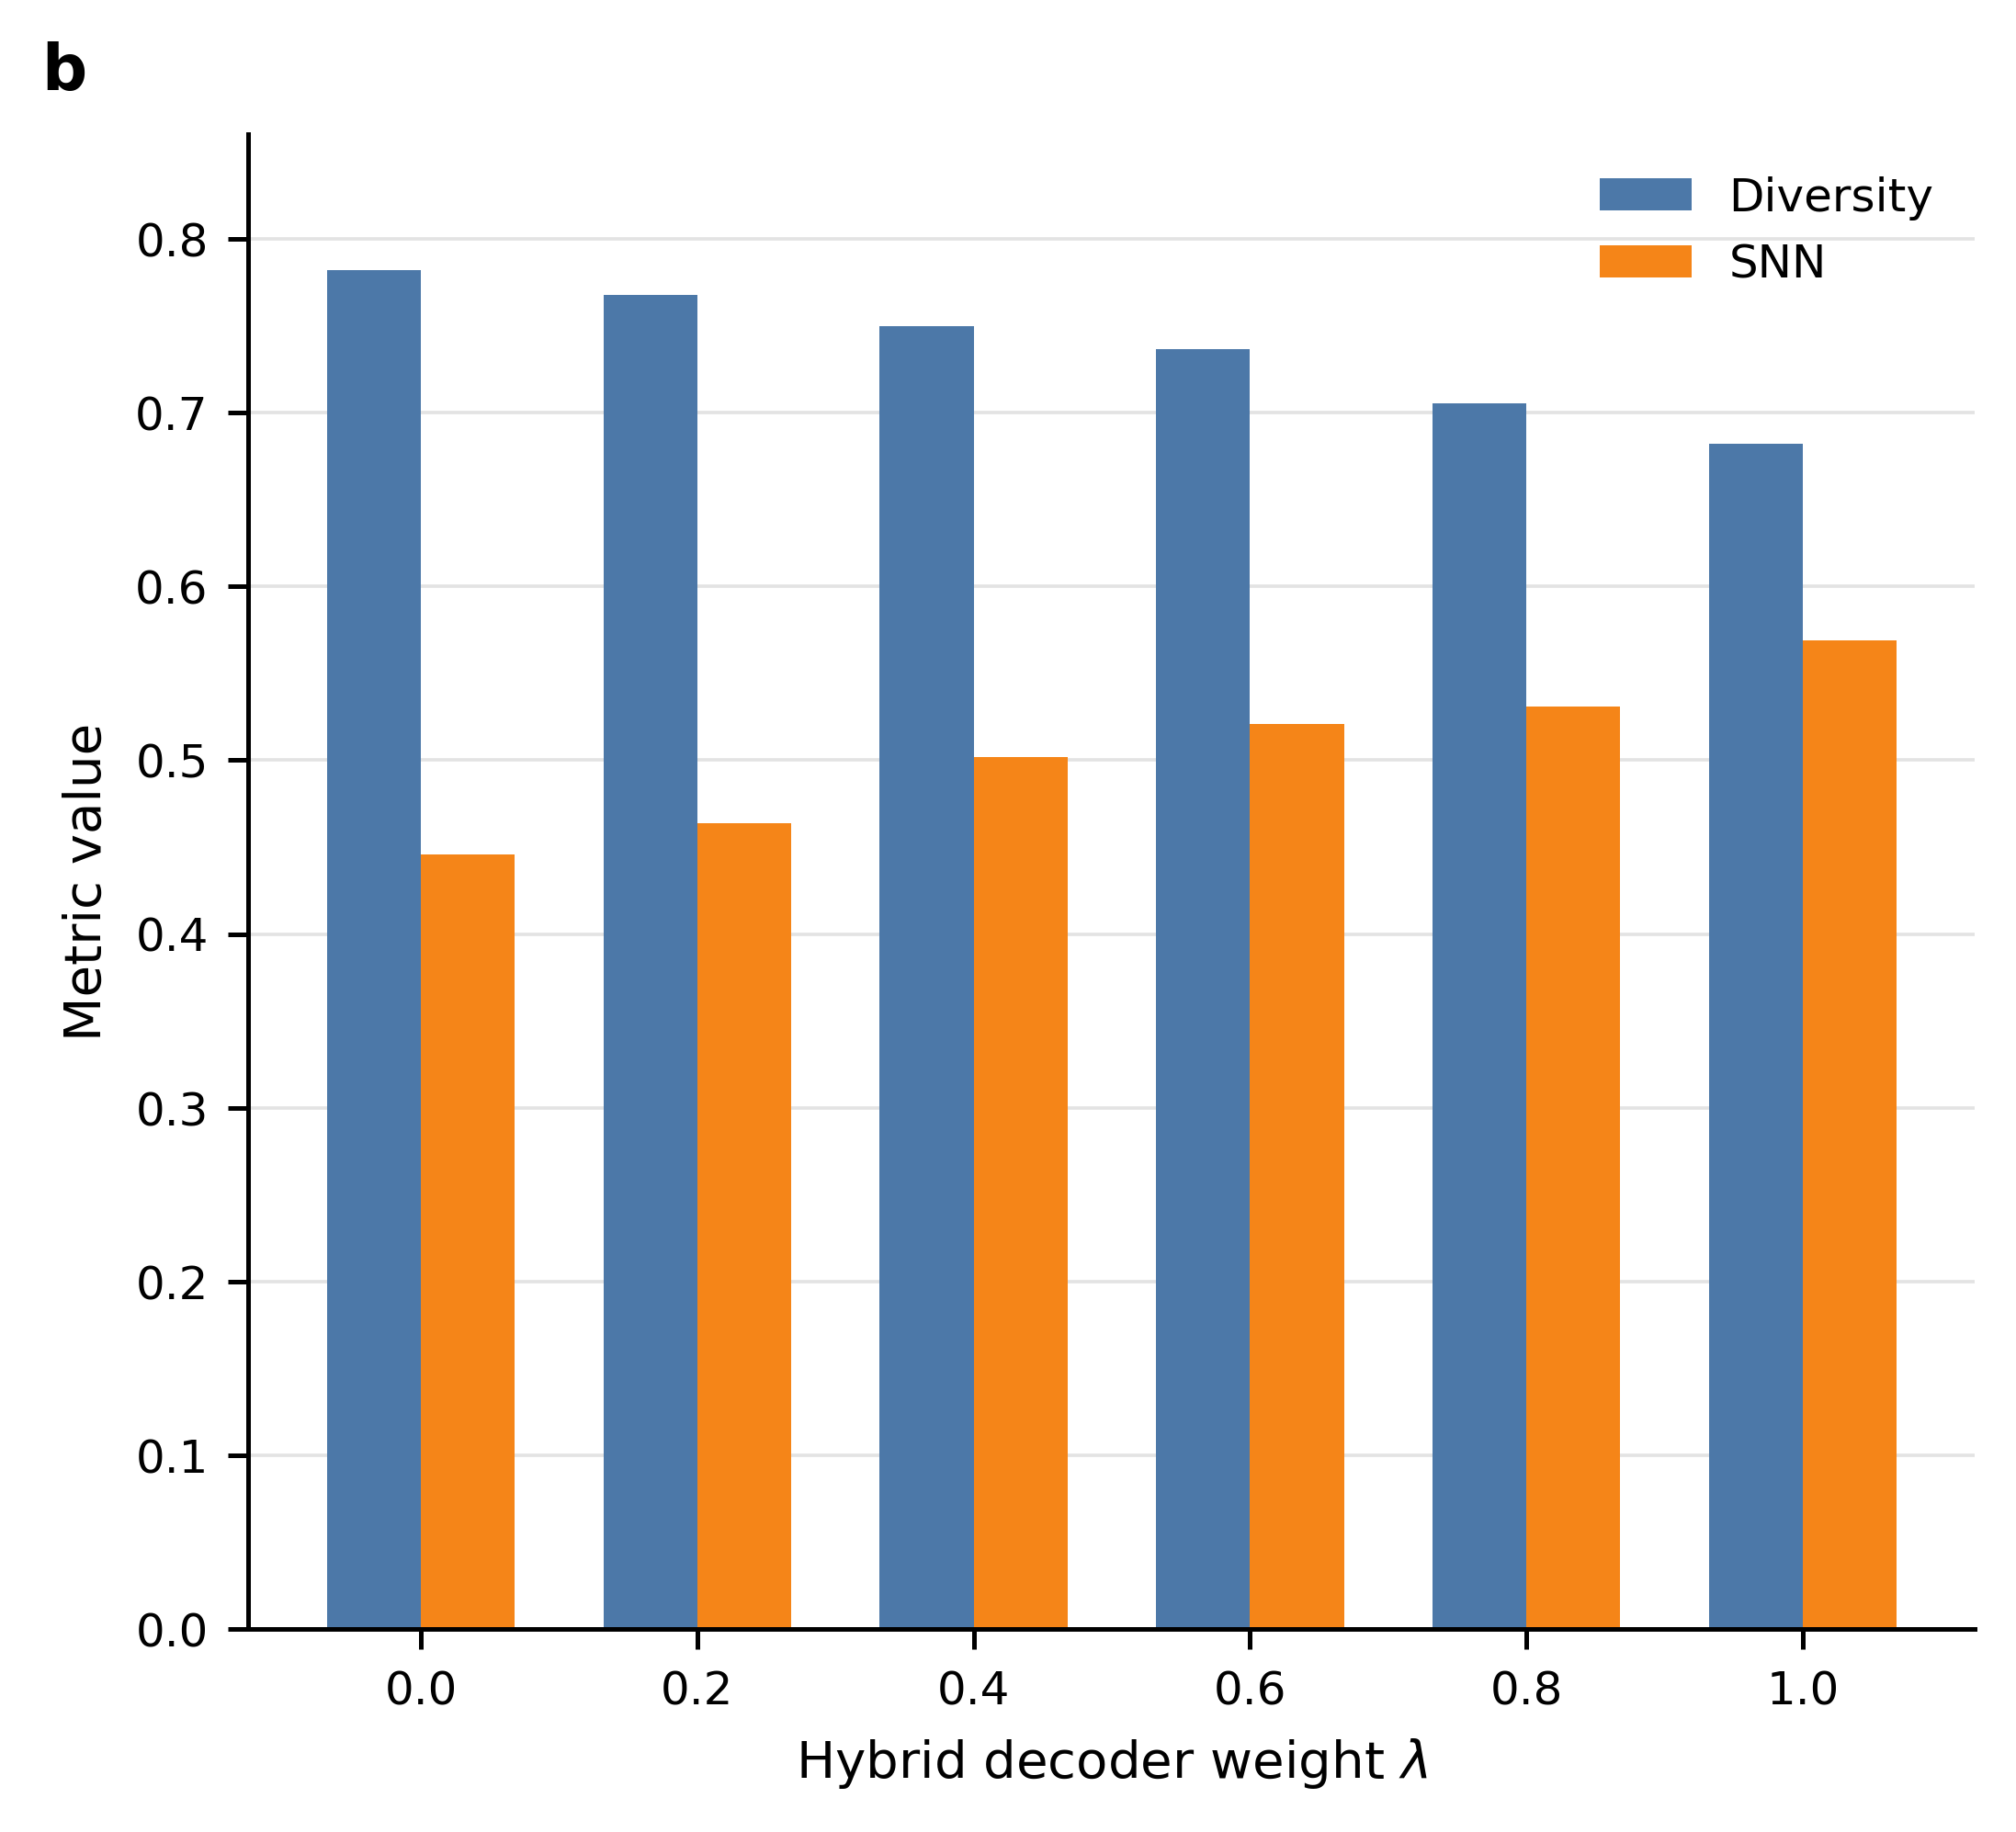
\includegraphics[width=0.58\textwidth]{result_data/figure2_b/figure2_b.png}
\caption{Diversity and SNN of PepALD generations under different hybrid-decoder fusion weights $\lambda$.}
\label{supfig:hybrid_lambda_sweep}
\end{figure}

\section{Permeability-training trajectory}
\label{supsec:permeability_training_trajectory}

\begin{figure}[h]
\centering
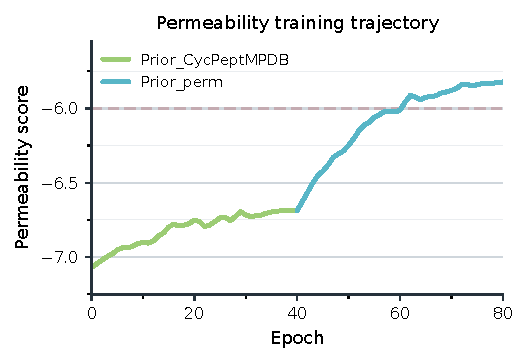
\includegraphics[width=0.70\textwidth]{result_data/figure_perm/fig3(b)_train/fig3b_train_curve.pdf}
\caption{Fitted mean-permeability trajectory across 40 epochs of cyclic-prior training followed by 40 epochs of permeability-oriented fine-tuning.}
\label{supfig:permeability_training_trajectory}
\end{figure}

\end{document}
